% ---
% Capa
% ---
\imprimircapa
% ---

% ---
% Folha de rosto
% (o * indica que haverá a ficha bibliográfica)
% ---
\imprimirfolhaderosto*
% ---

% ---
% Inserir a ficha bibliografica
% ---
% \begin{fichacatalografica}
% 	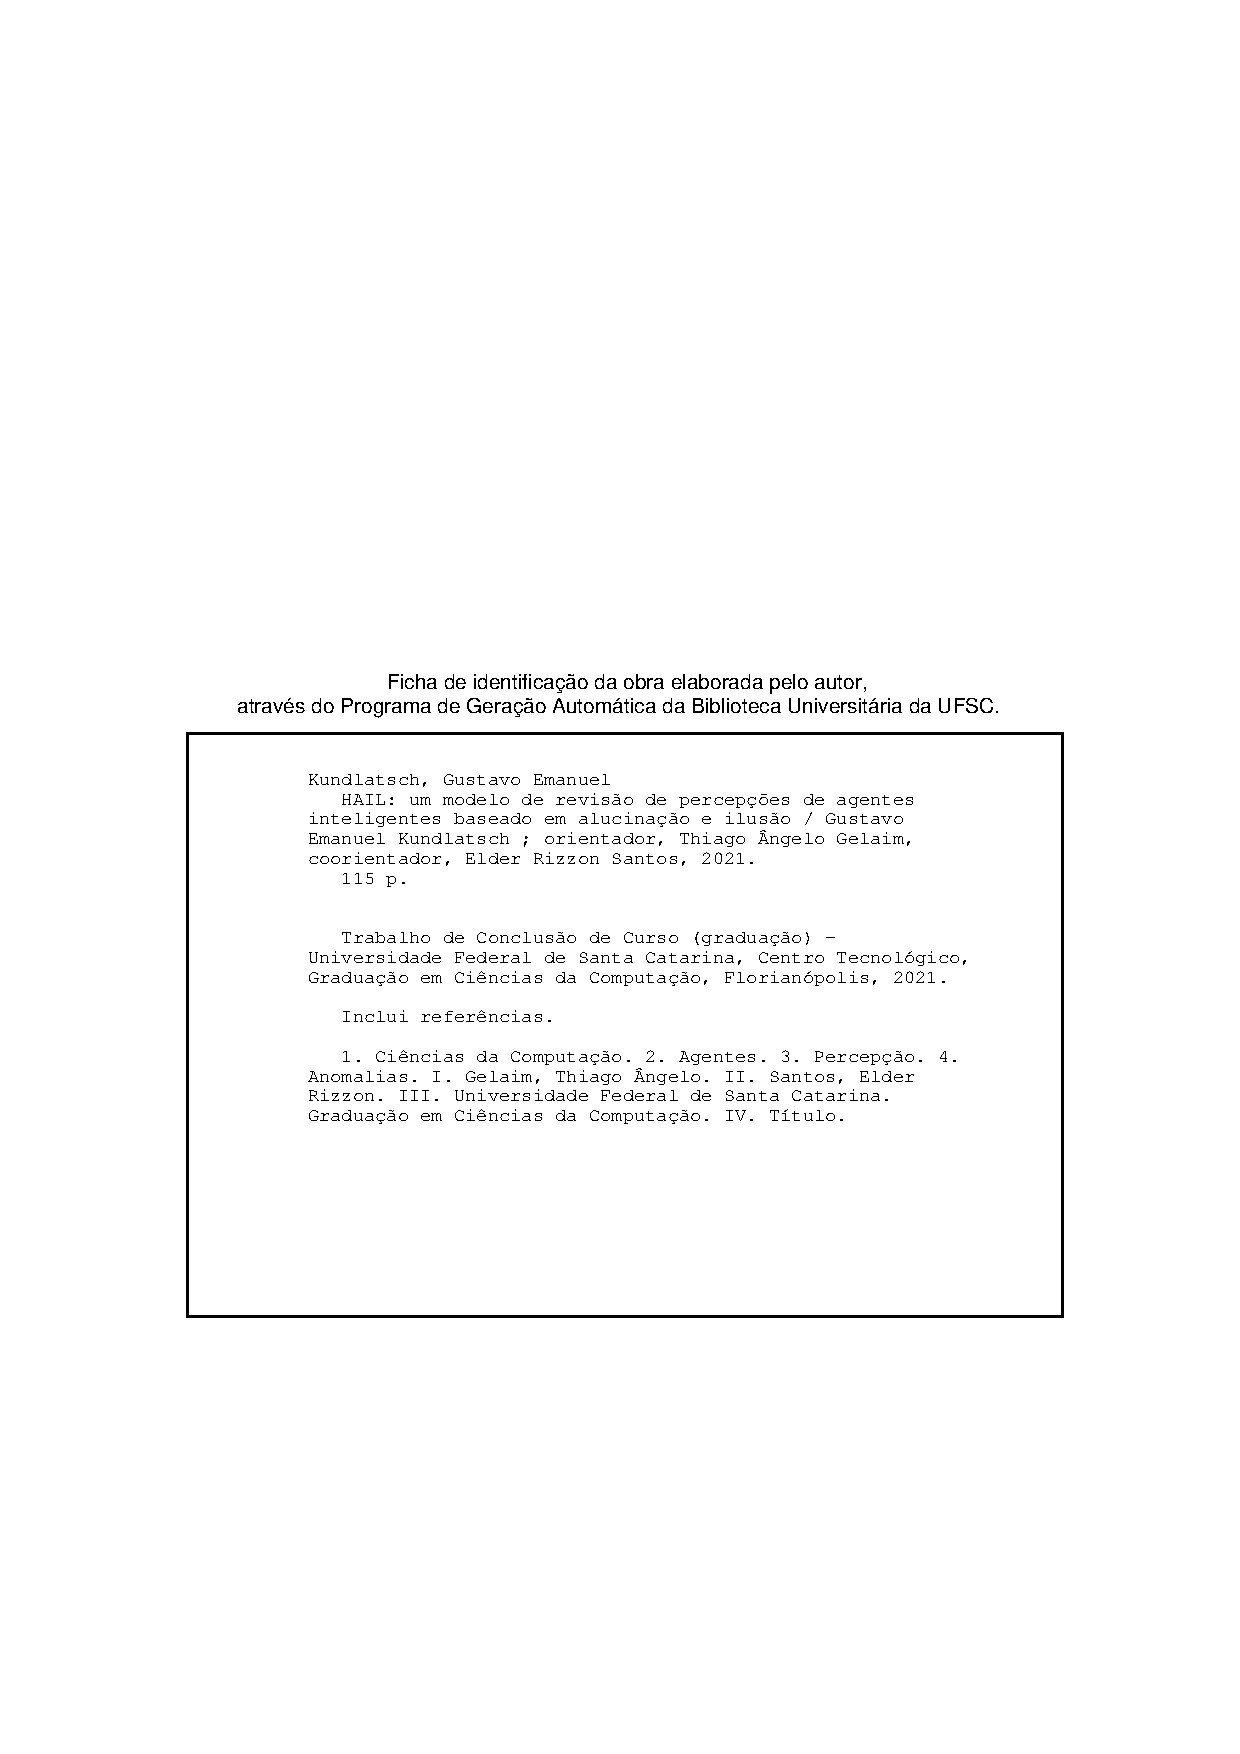
\includepdf{beforetext/Ficha_Catalografica.pdf}
% \end{fichacatalografica}
% ---

% ---
% Inserir folha de aprovação
% ---
% \begin{folhadeaprovacao}
% 	\OnehalfSpacing
% 	\centering
% 	\imprimirautor\\%
% 	\vspace*{10pt}		
% 	\textbf{\imprimirtitulo}%
% 	\ifnotempty{\imprimirsubtitulo}{:~\imprimirsubtitulo}\\%
% 	%		\vspace*{31.5pt}%3\baselineskip
% 	\vspace*{\baselineskip}
% 	%\begin{minipage}{\textwidth}
% 	O presente trabalho em nível de \imprimirnivel~foi avaliado e aprovado por banca examinadora composta pelos seguintes membros:\\
% 	%\end{minipage}%
% 	\vspace*{\baselineskip}
% 	Dr. Thiago Ângelo Gelaim\\
% 	Orientador\\
% 	\vspace*{\baselineskip}
% 	Prof. Dr. Elder Rizzon Santos \\
% 	Coorientador e Responsável\\
% 	\vspace*{\baselineskip}
% 	Prof. Dr. Rafael de Santiago\\
% 	\vspace*{\baselineskip}
% 	Me. Rodrigo Rodrigues Pires de Mello\\
% 	\vspace*{2\baselineskip}
% 	\begin{minipage}{\textwidth}
% 		Certificamos que esta é a \textbf{versão original e final} do trabalho de conclusão que foi julgado adequado para obtenção do título de \imprimirformacao.\\
% 	\end{minipage}
% 	%    \vspace{-0.7cm}
% 	\vspace*{\fill}
% 	\assinatura{\OnehalfSpacing Coordenação do Programa de Graduação}
% 	\vspace*{\fill}
% 	\assinatura{\OnehalfSpacing\imprimirorientador \\ \imprimirorientadorRotulo}
% 	%	\ifnotempty{\imprimircoorientador}{
% 	%	\assinatura{\imprimircoorientador \\ \imprimircoorientadorRotulo \\
% 	%		\imprimirinstituicao~--~\imprimirinstituicaosigla}
% 	%	}
% 	% \newpage
% 	\vspace*{\fill}
% 	\imprimirlocal, \imprimirano.
% \end{folhadeaprovacao}
% ---

% ---
% Dedicatória
% ---
\begin{dedicatoria}
	\vspace*{\fill}
	\noindent
	\begin{adjustwidth*}{}{5.5cm} 
		\raggedleft       
		À Maria, com amor. Minha companheira, amiga e por vezes revisora voluntária. Sua ajuda e motivação fez este trabalho comigo.
	\end{adjustwidth*}
\end{dedicatoria}
% ---

% ---
% Agradecimentos
% ---
\begin{agradecimentos}
    Agradeço a meus orientadores, sem os quais este trabalho não seria possível;
    Aos membros do SpaceLab, em especial a equipe do FloripaSat-2 pela ajuda e suporte;
    À minha família, especialmente minha mãe, que celebrou, reclamou, agradeceu e chorou comigo durante toda a graduação;
    À todos os servidores da UFSC, por manter e prover educação pública, gratuita e de qualidade;
\end{agradecimentos}
% ---

% ---
% Epígrafe
% ---
\begin{epigrafe}
	\vspace*{\fill}
	\begin{flushright}
		\textit{``O êxito precoce é um péssimo professor. Quando isso acontece, somos
                  recompensados por nossa falta de preparação e, quando nos vemos
                  no meio de uma situação para a qual devemos nos preparar, não somos capazes. Não sabemos como fazê-lo.'' \\
			(Chris Hadfield, An Astronaut's Guide to Life on Earth, 2013)}
	\end{flushright}
\end{epigrafe}
% ---

% ---
% RESUMOS
% ---

% resumo em português
\setlength{\absparsep}{18pt} % ajusta o espaçamento dos parágrafos do resumo
\begin{resumo}
	\SingleSpacing
	Satélites artificiais são projetos que demandam níveis elevados de confiabilidade de seus módulos. Apesar de alguns projetos permitirem atualizações posteriores a firmware e programas, são raros os casos onde é possível revisar e corrigir hardware. Por esse motivo a etapa de testes e AIV (\textit{Assembly, Integration, and Verification}) é crucial para a garantia de que o projeto não corra mais riscos do que os que são inerentes à área. Esses fatores são amplificados quando tratamos de \textit{CubeSats}, que possuem escopo e orçamentos menores quando comparados a grandes projetos governamentais e/ou comerciais. Este trabalho propõe a implementação de um sistema de \textit{workflows} hospedados na plataforma de controle de versionamento \textit{GitHub} que, aliados à funcionalidade GitHub Actions, permitirá a execução automatizada de testes no contexto dos planos de \emph{Assembly, Integration, and Verification}(AIV) da missão FloripaSat-2 e, posteriormente, análise e interpretação dos dados coletados de modo a obter resultados qualitativos e quantitativos da execução.
	
	
	\textbf{Palavras-chave}: CubeSat. Nanossatélite. FloripaSat-2. AIV.
\end{resumo}

% resumo em inglês
\begin{resumo}[Abstract]
	\SingleSpacing
	\begin{otherlanguage*}{english}
	    Artificial Satellites are projects that demand highly reliable modules. Despite some missions allowing post-deployment updates to firmware and software, cases where it is possible to perform hardware maintenance are rare. Because of this fact, the \textit{Assembly, Integration and Verification} (AIV) process is crucial to guarantee that the project doesn't face more risks than those which are inerent of a space mission. These factores are intensified when dealing with \textit{CubeSats}, that statistically have lower budgets and scope when compared to large scale governmental and/or commercial space missions. This article proposes the implementation of a test automation workflow system hosted at GitHub that will make use of the GitHub Actions tool to allow automated execution of tests during the AIV step of the FloripaSat-2 mission, and lastly, will allow collection and analysis of data in order to draw relevant conclusions regarding the execution.
	
	
		\textbf{Keywords}: CubeSat. Nanosatellite. FloripaSat-2. AIV.
	\end{otherlanguage*}
\end{resumo}
%% resumo em francês 
%\begin{resumo}[Résumé]
% \begin{otherlanguage*}{french}
%    Il s'agit d'un résumé en français.
% 
%   \textbf{Mots-clés}: latex. abntex. publication de textes.
% \end{otherlanguage*}
%\end{resumo}
%
%% resumo em espanhol
%\begin{resumo}[Resumen]
% \begin{otherlanguage*}{spanish}
%   Este es el resumen en español.
%  
%   \textbf{Palabras clave}: latex. abntex. publicación de textos.
% \end{otherlanguage*}
%\end{resumo}
%% ---

{%hidelinks
	\hypersetup{hidelinks}
	% ---
	% inserir lista de ilustrações
	% ---
	\pdfbookmark[0]{\listfigurename}{lof}
	\listoffigures*
	\cleardoublepage
	% ---
	
	% ---
	% inserir lista de quadros
	% ---
	\pdfbookmark[0]{\listofquadrosname}{loq}
	\listofquadros*
	\cleardoublepage
	% ---
	
	% ---
% 	inserir lista de tabelas
% 	% ---
	\pdfbookmark[0]{\listtablename}{lot}
	\listoftables*
	\cleardoublepage
	% ---
	
	
	% ---
	% inserir lista de abreviaturas e siglas (devem ser declarados no preambulo)
	% ---
	% ---------------------------------------------------
% ------ Lista de abreviaturas e siglas -------------
% ---------------------------------------------------

\begin{siglas}
  \item[ AIV ] \emph{Assembly, Integration, and Verification}
  \item[ CSA ] \textit{Canadian Space Agency}
  \item[ FlatSat ] Plataforma de testes para módulos CubeSat
  \item[ NASA ] \textit{National Aeronautics and Space Administration}
  \item[ SpaceLab ] Laboratório de Pesquisa em Tecnologias Espaciais - UFSC
  \item[ UFSC ] Universidade Federal de Santa Catarina
\end{siglas}
	% ---
	
	% ---
	% inserir lista de símbolos (devem ser declarados no preambulo)
	% ---
% 	% ---------------------------------------------------
% ----------- Lista de símbolos ---------------------
% ---------------------------------------------------

\begin{simbolos}
%   \item[$ \Delta $] Função de transição do modelo de revisão de percepções
%   \item[$ \Gamma $] Função de transição que especifica um sistema de transição de estados $\Sigma$
%   \item[$ \gamma $] Função de percepção do agente
%   \item[$ \theta $] Função de refinamento
%   \item[$ \rho $] Conjunto de percepções refinadas
%   \item[$ \Sigma $] Sistema de transição de estados de um modelo conceitual de planejamento automatizado
%   \item[$ \Psi $] Conjunto união formado pelas pré-condições das ações que compõem um plano
%   \item[$ \psi $] Conjunto de pré-condições de uma ação
%   \item[$ \Omega $] Conjunto união formado pelas pós-condições das ações que compõem um plano
%   \item[$ \omega $] Conjunto de pós-condições de uma ação
%   \item[$ A $] Conjunto finito ou recursivamente enumerável de ações
%   \item[$ Ab $] Conjunto de blocos avaliadores
%   \item[$ Ab_{h} $] Bloco avaliador de alucinações
%   \item[$ Ab_{i1} $] Bloco avaliador de ilusões classe 1
%   \item[$ Ab_{i2} $] Bloco avaliador de ilusões classe 2
%   \item[$ Ag$ ] Agente
%   \item[$ Ap $] Conjunto de blocos de planejamento automatizado
%   \item[$ Ap_{h} $] Bloco de planejamento automatizado de alucinações
%   \item[$ Ap_{i} $] Bloco de planejamento automatizado de ilusões
%   \item[$ c $] Contexto do agente
%   \item[$ Ce $] Função equação de limpeza do bloco avaliador
%   \item[$ Cf $] Função de limpeza do bloco avaliador
%   \item[$ D $] Conjunto de decisores
%   \item[$ d_{a} $] Decisor de anomalias
%   \item[$ d_{h} $] Decisor de alucinações
%   \item[$ d_{i} $] Decisor de ilusões
%   \item[$ E $] Conjunto finito ou recursivamente enumerável de eventos
%   \item[$ K $] Conjunto de conhecimentos do agente
%   \item[$ L $] Lista ordenada
%   \item[$ |L| $] Número de elementos de uma lista ordenada
%   \item[$ L_i $] Elemento $i$ da lista ordenada $L$
%   \item[$ M_{ai} $] Módulo de alucinação e ilusão
%   \item[$ P $] Conjunto de planos do agente
%   \item[$ p $] Conjunto de percepções iniciais
%   \item[$ P(L_i) $] Função peso da lista ponderada
%   \item[$ Pf $] Função de processamento do bloco avaliador
%   \item[$ S $] Conjunto finito ou recursivamente enumerável de estados
%   \item[$ T_{m}(x) $] Função tempo médio de x
%   \item[$ W $] Função peso de uma anomalia
%   \item[$ Z $] Descrição de sistema
\end{simbolos}


	% ---
	
	% ---
	% inserir o sumario
	% ---
	\pdfbookmark[0]{\contentsname}{toc}
	\tableofcontents*
	\cleardoublepage
	
}%hidelinks
% ---